\section{Results}
\label{sec:results}

\subsection{Historical Cross-Platform Context}
\label{sec:historical-context}
The original 32~MiB AES-128-CTR campaign reported median host-relative
prepared-pipeline speedups of $0.935\times$ on the GTX 1650 Ti,
$1.354\times$ on the T600, and $4.761\times$ on the Tesla T4.
Those measurements used PyCryptodome host calls and include differences
in software versions, CPU dispatch, platform scheduling and API scope.
The result establishes that measured offload advantage varied between the
three complete configurations; it does \emph{not} establish that the T4
outperforms a native OpenSSL CPU transform. The updated same-runtime
comparison below resolves that ambiguity. Earlier ECB, small-buffer and
throughput observations remain in the reproducibility archive and are not
used to infer page-workload effects.


Table~\ref{tab:gpu-speedups} preserves the historical 32~MiB
mode comparison, including resident and transfer-inclusive outcomes.
It is presented for context, not as a pooled analysis with the later
T4/OpenSSL campaign. The T600 and T4 CTR configurations favored the
GPU under their original PyCryptodome-based boundaries; the GTX result
was near parity. Those historical results therefore motivate--rather
than replace--the optimized-host experiment.

\begin{table}[htbp]
  \centering
  \small
  \setlength{\tabcolsep}{4pt}
  \caption{Paired speedup over AES-NI at 32~MiB. R: resident; P: pipeline.
  Brackets show the five-session pipeline range; the last column counts P gains.}
  \label{tab:gpu-speedups}
  \begin{tabular}{llrrlc}
    \toprule
    System & Mode & R & P & P range & P $>1$ \\
    \midrule
    GTX & ECB & 3.091 & 0.761 & [0.722, 0.818] & 0/5 \\
    GTX & CTR & 3.693 & 0.935 & [0.918, 1.008] & 1/5 \\
    T600 & ECB & 2.215 & 1.118 & [0.659, 1.144] & 3/5 \\
    T600 & CTR & 2.666 & 1.354 & [1.129, 1.391] & 5/5 \\
    T4 & ECB & 2.207 & 0.893 & [0.868, 0.901] & 0/5 \\
    T4 & CTR & 11.758 & 4.761 & [4.691, 5.021] & 5/5 \\
    \bottomrule
  \end{tabular}
\end{table}


Figure~\ref{fig:bulk-throughput} provides the absolute throughput
counterpart to those ratios. The differences between resident and
prepared-pipeline rates illustrate why a peak kernel figure alone does
not determine a complete host-to-host encryption rate.

\begin{figure}[htbp]
\centering
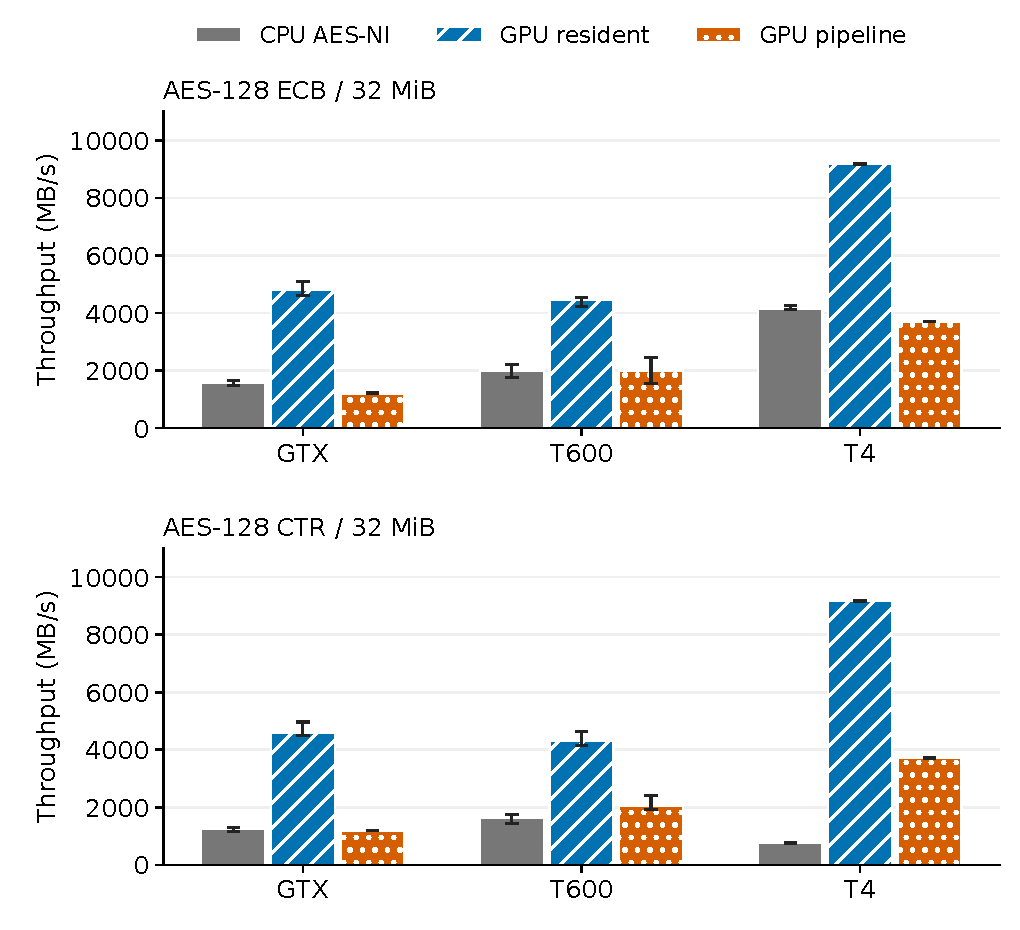
\includegraphics[width=0.95\linewidth]{figures/bulk_throughput.pdf}
\caption{Historical 32~MiB AES-128 throughput for three complete
configurations. CPU references use the original PyCryptodome paths;
resident GPU timing excludes host--device transfers, whereas the
prepared pipeline includes synchronous payload transfers. These data
are not paired with the later OpenSSL-controlled campaign.}
\label{fig:bulk-throughput}
\end{figure}

\subsection{Oracle Cloud ARM64: CPU Implementation and Envelope Controls}
\label{sec:oracle-results}
On the independent Oracle Cloud ARM64 host, the five-session 32~MiB
AES-128-CTR study produced approximately 4.03~GB/s of native
OpenSSL-default transform-only throughput, compared with approximately
209~MB/s for the PyCryptodome path and 218~MB/s for the
\texttt{OPENSSL\_armcap=0} control. These values describe the specific
library implementations and timed boundaries; they are not GPU speedups.
The default OpenSSL path was approximately 19.3 times faster than the
recorded PyCryptodome transform path at this size, with the important
qualification that Python/FFI and C-native interval definitions differ.

In a separate host-side envelope experiment, a single worker achieved
approximately 1.06~GB/s at 32~MiB, while two concurrent workers reached
approximately 2.03~GB/s in aggregate, or about 1.92 times the
single-worker aggregate rate. These campaigns are not paired
per-repetition observations and their envelope boundary differs from the
4.03~GB/s native transform interval. The contrast demonstrates that
buffer lifecycle and concurrency must be considered before extending
cryptographic core throughput to a complete service. No Oracle result is
used to calculate a speedup against the Tesla T4 or other GPU system.

\subsection{Revisiting the Host Baseline on the Tesla T4}
\label{sec:new-t4-baseline}
The historical $4.761\times$ T4 CTR speedup in the preceding tables is an
\emph{earlier PyCryptodome-relative result}, not a speedup relative to an
optimized native OpenSSL implementation. In a new five-session T4 campaign,
32~MiB AES-128-CTR yields a $5.586\times$ median session ratio against
PyCryptodome but only $0.942\times$ against native OpenSSL when the GPU
prepared pipeline is the denominator. The OpenSSL transform throughput is
approximately 3.874~GB/s and the GPU prepared-pipeline throughput is
approximately 3.646~GB/s. When only GPU resident computation is considered,
the native OpenSSL CPU/GPU ratio is $2.299\times$. Thus the improved CPU
baseline reverses the prepared-pipeline ranking, without implying that the
historical measurements were incorrect.

\subsection{Independent Pages: A Compute Advantage That Does Not Survive Transfers}
\label{sec:page-results}
Table~\ref{tab:page-primary} gives the prespecified native OpenSSL transform
to prepared CUDA pipeline time ratios in the page-batching study. Every
reported ratio is below unity across all five sessions. The gap narrows at
larger batch sizes but does not reverse direction.

\begin{table}[htbp]
\centering\small
\caption{Tesla T4 Phase 2: median of five session-level CPU OpenSSL transform / GPU prepared-pipeline ratios. Values below one favor the CPU at this boundary.}
\label{tab:page-primary}
\begin{tabular}{@{}rrr@{}}\toprule
Total payload & Continuous CTR & Independent 1~MiB pages\\\midrule
1~MiB & 0.5437 & 0.5404\\
4~MiB & 0.6948 & 0.7137\\
16~MiB & 0.8163 & 0.8240\\
32~MiB & 0.8963 & 0.9125\\\bottomrule
\end{tabular}
\end{table}

The most informative case is a batch of 32 independent pages. The median CPU
native transform duration is approximately 8.362~ms, compared with 3.714~ms
for one GPU-resident kernel and 9.153~ms for the prepared GPU pipeline.
Table~\ref{tab:page-32-components} separates the measurements. The
compute-only ratio is $2.251\times$ in favor of the GPU, whereas the
transfer-inclusive ratio is $0.913\times$ and favors the CPU. Both directions
are consistent across all five sessions. The observed H2D-plus-D2H component
is about 5.418~ms. Medians of nested or separately timed components cannot
be added as if they described a single observation.

\begin{table}[htbp]
\centering\small
\caption{Tesla T4 Phase 2, 32 independent 1~MiB pages: separately summarized timings (five session medians).}
\label{tab:page-32-components}
\begin{tabularx}{\linewidth}{@{}Xr@{}}\toprule
Measurement boundary & Approximate time (ms)\\\midrule
Native OpenSSL CPU transform & 8.362\\
CUDA resident kernel & 3.714\\
GPU H2D + D2H transfers & 5.418\\
CUDA prepared pipeline, including transfers and synchronization & 9.153\\\midrule
GPU compute-only speedup versus CPU transform & $2.251\times$\\
GPU prepared-pipeline speedup versus CPU transform & $0.913\times$\\\bottomrule
\end{tabularx}
\end{table}

\begin{figure}[htbp]
\centering
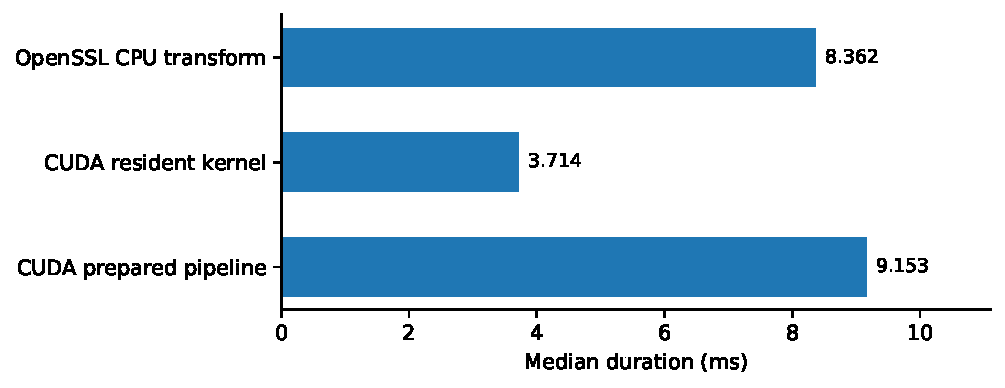
\includegraphics[width=0.89\linewidth]{figures/page_32_boundary_comparison.pdf}
\caption{Observed 32~MiB independent-page timing at three explicitly
different boundaries. Each bar represents the median of five session
medians; the GPU resident bar excludes host--device transfers, while
the prepared-pipeline bar includes them. The figure compares measured
intervals, not identical application-level API calls.}
\label{fig:page-32-boundaries}
\end{figure}

The page-aware GPU prepared pipeline shows almost no relative penalty against
a single continuous CTR stream of the same size: its page/continuous
throughput ratios are approximately $1.0007\times$ at 4~MiB,
$1.0068\times$ at 16~MiB and $1.0066\times$ at 32~MiB. These sub-percent
differences should not be described as a robust optimization gain. They
support the narrower observation that independent per-page counter handling
does not impose a large measured GPU pipeline overhead in the evaluated
implementation. This is distinct from demonstrating an advantage from
batching over sequential per-page GPU launches, which was not the control
experiment.
